\setlength{\columnsep}{3pt}
\begin{flushleft}

\bigskip
\begin{itemize}
	\item On a server with 6 cores and 2 threads per core (total of 12 CPUs), the usage could go up to 1200\%. 
	\bigskip
	\item \textbf{Command to display process by maximum CPU consumption:}
	\bigskip
	\begin{tcolorbox}[breakable,notitle,boxrule=-0pt,colback=pink,colframe=pink]
		\color{black}
		\fontdimen2\font=1em
		Syntax: top
		\newline
		\color{blue}
		Press "P" to sort task list by processor usage
		\fontdimen2\font=4pt
	\end{tcolorbox}
	Eg:
	\begin{figure}[h!]
		\centering
		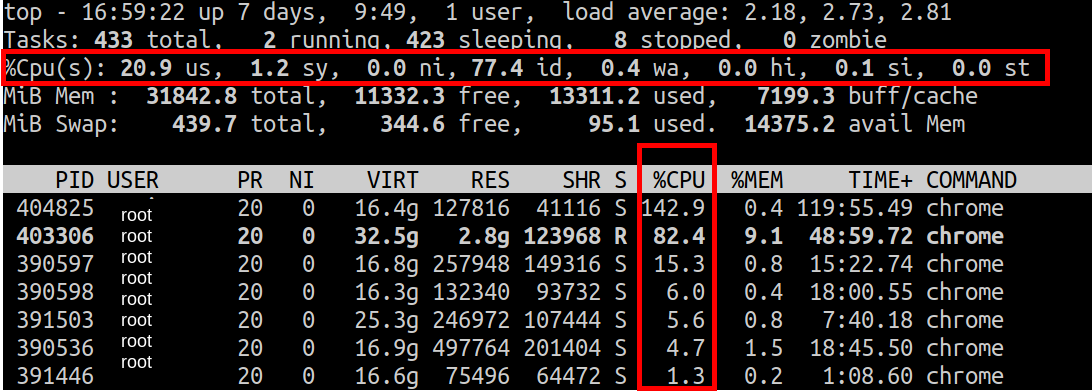
\includegraphics[scale=.32]{content/chapter12/images/top_2.png}
		\caption{Sample output}
		\label{fig:cpu2}
	\end{figure}

	In "top" what are us, sy, ni, id, wa, hi, si and st (for CPU usage)?
	\begin{itemize}
		\item us - \%CPU time spent in user space
		\item sy - \%CPU time spent in kernel space
		\item ni - \%CPU time spent on low priority processes
		\item id - \%CPU time spent idle
		\item wa - \%CPU time spent in wait (on disk)
		\item hi - \%CPU time spent with hardware interrupts
		\item si - \%CPU time spent with software interrupts
		\item st - \%CPU time stolen from a virtual machine
	\end{itemize}
	
	
	
	
\end{itemize}


\end{flushleft}

\newpage


